\documentclass[12pt]{article}            % Report class in 11 points
\parindent0pt  \parskip12pt             % make block paragraphs
\usepackage{graphicx}
\usepackage{listings}
\graphicspath{ {images/} }
\usepackage{graphicx} %  graphics header file
\begin{document}
\begin{titlepage}
    \centering
  \vfill
    
\includegraphics[width=8cm]{uni_logo.png} \\ 
	\vskip2cm
    {\bfseries\Large
	Data Structures and Algorithms \\ (CS09203)\\
	
	\vskip2cm
	Lab Report 
	 
	\vskip2cm
	}    

\begin{center}
\begin{tabular}{ l l  } 

Name: & Rehman ullah baig \\ 
Registration \#: &CSU-F16118 \\ 
Lab Report \#: & 09 \\ 
 Dated:& 11-06-2018\\ 
Submitted To:& Mr. Usman Ahmed\\ 

 %\hline
\end{tabular}
\end{center}
    \vfill
    The University of Lahore, Islamabad Campus\\
Department of Computer Science \& Information Technology
\end{titlepage}


    
    {\bfseries\Large
\centering
	Experiment \# 9 \\

The Depth-first search algorithm\\
	
	}    
 \vskip1cm
 \textbf {Objective}\\  To understand and implement The Depth-first search algorithm.
 
 \textbf {Software Tool} \\
1. Windows 7  \\
2. Dev C++\\
3. Miktex   \\

\section{Theory }              
A standard DFS implementation puts each vertex of the graph into one of two categories:

Visited
Not Visited
The purpose of the algorithm is to mark each vertex as visited while avoiding cycles. \\
The DFS algorithm works as follows:\\
1.	Start by putting any one of the graph's vertices on top of a stack.\\
2.	Take the top item of the stack and add it to the visited list.\\
3.	Create a list of that vertex's adjacent nodes. Add the ones which aren't in the visited list to the top of stack.\\ \\
3.	Keep repeating steps 2 and 3 until the stack is empty.\\ \\

\section{Task}  
\subsection{Procedure: Task 1 }     

\begin{figure*}
\centering
  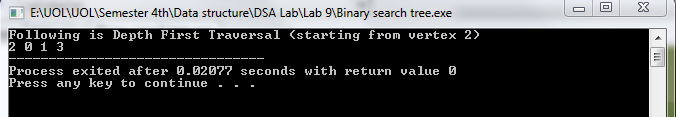
\includegraphics[width=12cm,height=6cm,keepaspectratio]{2.png}
\caption{Data entering into different locations}
\label{Figure:3}    
\end{figure*}
Tin the following graph, we start traversal from vertex 2. When we come to vertex 0, we look for all adjacent vertices of it. 2 is also an adjacent vertex of 0. If we don’t mark visited vertices, then 2 will be processed again and it will become a non-terminating process. A Depth First Traversal of the following graph is 2, 0, 1, 3

\subsection{Procedure: Task 2 }     

\begin{lstlisting}[language=C++]

#include<iostream>
#include<list>
using namespace std;
class Graph
{
    int V;    
 
    list<int> *adj;
 
    void DFSUtil(int v, bool visited[]);
public:
    Graph(int V);   
 
    void addEdge(int v, int w);
 
    void DFS(int v);
};
 
Graph::Graph(int V)
{
    this->V = V;
    adj = new list<int>[V];
}
 
void Graph::addEdge(int v, int w)
{
    adj[v].push_back(w); 
}
 
void Graph::DFSUtil(int v, bool visited[])
{
    visited[v] = true;
    cout << v << " ";
    list<int>::iterator i;
    for (i = adj[v].begin(); i != adj[v].end(); ++i)
        if (!visited[*i])
            DFSUtil(*i, visited);
}
 
void Graph::DFS(int v)
{
    bool *visited = new bool[V];
    for (int i = 0; i < V; i++)
        visited[i] = false;
 
    DFSUtil(v, visited);
}
 
int main()
{
    Graph g(4);
    g.addEdge(0, 1);
    g.addEdge(0, 2);
    g.addEdge(1, 2);
    g.addEdge(2, 0);
    g.addEdge(2, 3);
    g.addEdge(3, 3);
 
    cout << "Following is Depth First Traversal"
            " (starting from vertex 2) \n";
    g.DFS(2);
 
    return 0;
}
\end{lstlisting}

\section{Conclusion}  
Depth first search is an interesting algorithm, and as you might suspect, it is particularly well suited for inspecting if a graph is connected; if the tree returned by depth first search contains all vertices in the graph, it is connected, otherwise, it is not.

 
\end{document}                          % The required last line
